\documentclass[12pt,oneside,a4paper,english]{article}
\usepackage[T1]{fontenc}
\usepackage[utf8]{inputenc} % Changed from latin2 to utf8 for better compatibility
\usepackage[margin=2.25cm,headheight=26pt,includeheadfoot]{geometry}
\usepackage[english]{babel}
\usepackage{listings}
\usepackage{color}
\usepackage{titlesec}
\usepackage{titling}
\usepackage[framed, numbered]{matlab-prettifier}
\usepackage{changepage}
\usepackage{amsmath}
\usepackage{hyperref}
\usepackage{enumitem}
\usepackage{graphicx}
\usepackage{fancyhdr}
\usepackage{lastpage}
\usepackage{caption}
\usepackage{tocloft}
\usepackage{setspace}
\usepackage{multirow}
\usepackage{titling}
\usepackage{float}
\usepackage{comment}
\usepackage{booktabs}
\usepackage{indentfirst}
\usepackage{lscape}
\usepackage{booktabs,caption}
\usepackage[flushleft]{threeparttable}
\usepackage[english]{nomencl}
\usepackage{xcolor}
\usepackage{lipsum}

% Set up hyperref
\hypersetup{
    colorlinks=true,
    linkcolor=blue,
    filecolor=magenta,      
    urlcolor=cyan,
    pdftitle={Aldebaran Transit Near Venus in 2025},
    pdfpagemode=FullScreen,
}

% --- set footer and header ---
\pagestyle{fancy}
\fancyhf{}
\rhead{Aldebaran Transit Near Venus}
\lhead{Astronomical Observation}
\rfoot{Page \thepage\ of \pageref{LastPage}}

% --- Title formatting ---
\title{\textbf{Aldebaran Transit Near Venus in 2025}}
\author{Astronomy Enthusiast}
\date{\today}

% --- Fix typo in Aldebaran throughout document ---
\newcommand{\Aldebaran}{Aldebaran}

% --- End of page settings ---
\begin{document}
\maketitle

\begin{abstract}
This article describes the upcoming close approach of \Aldebaran\ and Venus on July 13th, 2025. The event will be visible from the northern hemisphere and represents a rare astronomical alignment worth observing.
\end{abstract}

\section{Introduction}
This article outlines the upcoming close approach of \Aldebaran\ and Venus on July 13th, 2025. The event will be visible from the northern hemisphere and will be the first such close conjunction in over 100 years. 

\begin{figure}[H]
\centering
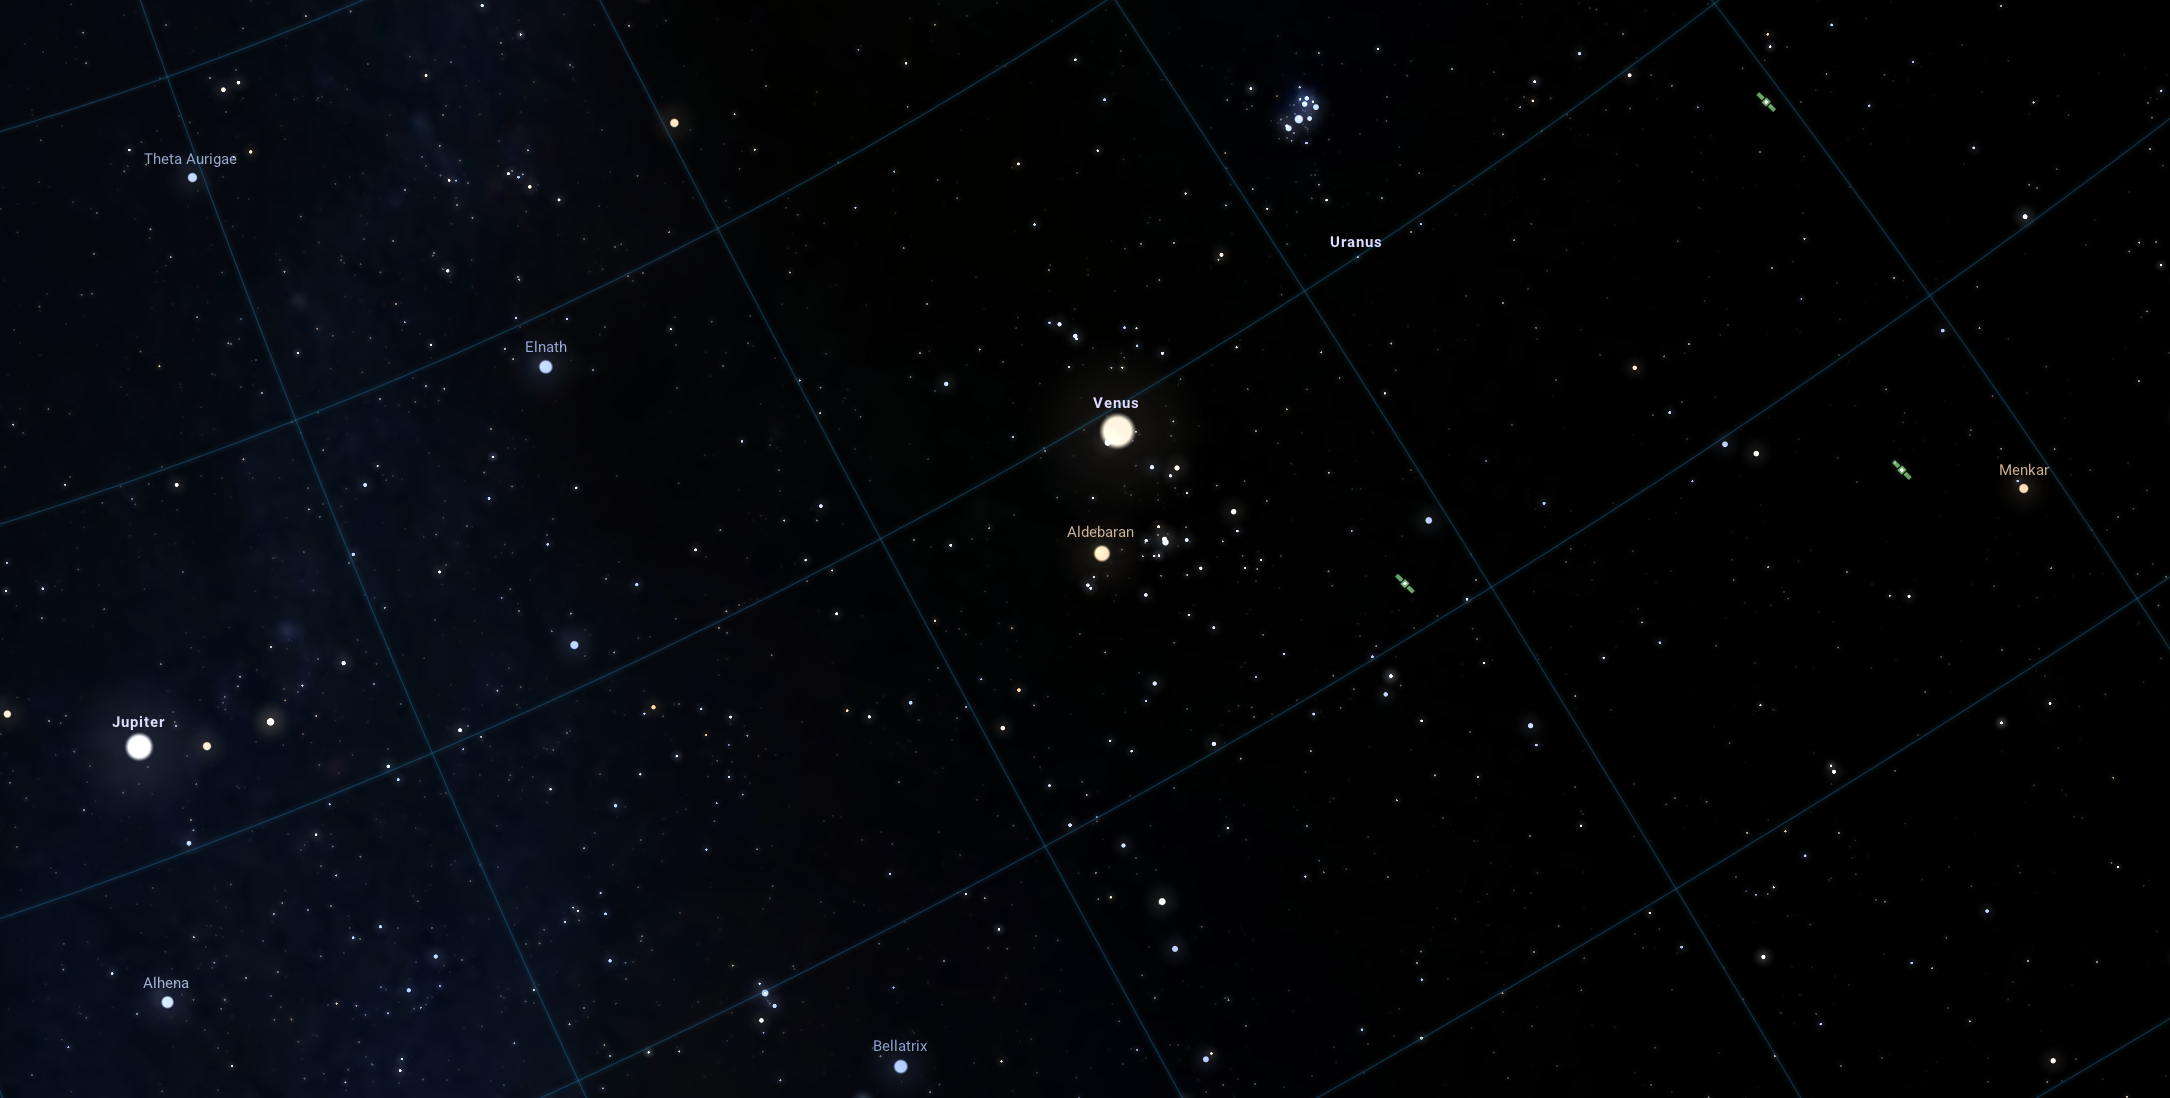
\includegraphics[width=0.8\textwidth]{VenusTransit.png}
\caption{Stellarium Web Map showing Venus and \Aldebaran\ on July 13th, 2025 from \href{https://stellarium-web.org/}{Stellarium Web}.}
\label{fig:venus_transit}
\end{figure}

\section{Recommended Equipment and Viewing Notes}
\Aldebaran\ and Venus are both visible to the naked eye, with \Aldebaran\ being the brightest star in the Taurus constellation. The event will be visible from most of Europe, Asia, and North America. 

Key viewing details:
\begin{itemize}
\item Start time: 10:00 UTC
\item Duration: Approximately 6 hours
\item Optimal viewing window: 10:00 to 16:00 UTC
\item Location: Northern Hemisphere (look for the Taurus constellation)
\end{itemize}

\section{Physics of the Event}
While the close approach of Venus and \Aldebaran\ is a rare alignment, it's important to note the different nature of these objects:

\begin{itemize}
\item Venus is within our solar system (average distance from Earth: 0.28 AU)
\item \Aldebaran\ is a distant star (65.3 light-years away)
\end{itemize}

The proper motion of Venus is significantly greater than that of \Aldebaran. Proper motion refers to the apparent movement of celestial objects as observed from Earth. The closer an object is, the more apparent its motion across the night sky will be (read more at: \href{https://en.wikipedia.org/wiki/Proper_motion}{Proper Motion}).

During observation, note these distinguishing features:
\begin{itemize}
\item \Aldebaran\ will shimmer due to atmospheric scintillation (twinkling)
\item Venus will appear as a steady, non-twinkling point of light
\end{itemize}

\section{Conclusion}
The motion of planets was a mystery for many years until the heliocentric model was proposed by Copernicus. Planetary movements have held significant importance in both astrology and astronomy throughout human history. This event continues the tradition of careful observation of our night sky. The 2025 close approach of Venus and \Aldebaran\ presents an excellent opportunity for both amateur and professional astronomers to observe a rare celestial alignment. Such events remind us of the dynamic nature of our solar system and its place within the broader galaxy.

\section*{Additional Resources}
\begin{itemize}
\item NASA's Sky Events Calendar: \url{https://science.nasa.gov/skywatching/}
\item International Astronomical Union: \url{https://www.iau.org/}
\item Stellarium Astronomy Software: \url{https://stellarium.org/}
\end{itemize}

\end{document}